\chapter{绪论}\label{chap:introduction}
随着人工智能技术的快速发展,人们的生活方式已经发生了许多变化:从现金结账到刷脸支付,从公共交通到自动驾驶,从人工咨询到智能客服,
从营销员推销式购物到无人零售,从洗衣拖地到智能家居。这些都是过去几年科技的发展给
人类生活带来的影响。这些改变的背后都喻示着技术的发展,其中尤为重要的一个就是
人工智能技术。其实``人工智能''的概念并不是近几年才出现的,早在1956年就有科学家
想用当时才刚刚出现不久的计算机来构建出具有人类智能的机器。
人工智能的概念就诞生于此,但这之后也没有引起多大的反响,只有少数感兴趣的人将它当作研究目标
默默在实验室耕耘。再后来的几十年间,人工智能就这样慢慢酝酿,不温不火,它一方面
代表了科学家们的美好愿景,一方面被技术人员视为空中楼阁。
直到2012年深度学习出现,伴随着逐年增长的数据量,以及越来越廉价的计算资源,
人工智能才又一次走入大众视野。
%根据相关平台报告,截至2017年第一季度,在全球范围内,人工智能相关专业技术人才总量超过190万,
%中国地区人工智能领域专业人才超过5万人,并且还存在500多万的人才缺口。
%可见人工智能领域的发展造成了相关专业人才短缺,供不应求。
据领英大数据显示,早在2017年全球人工智能领域人才已经突破190万,仅中国地区就有超过5万的相关专业人才,而且还存在500多万的人才缺口。可见人才培养速度已经落后于人工智能的发展速度,所以造成供不应求的局面。
再人工智能飞速发展的同时,其所涵盖的范围也在不断扩张,除了早期的机器学习,现在的研究领域还包括专家系统、
机器感知、推荐系统等。
图~\ref{fig:ai}给出了人工智能的一些分支。其中机器学习可以看作实现人工智能的
一种方法,它通过特定算法在数据集上进行训练,进而学习到数据的特征,最后达到
对未知样本做出决策或预测的效果。
% 与此同时,人工智能的研究领域也在不断扩大,图~\ref{fig:ai}展示了人工智能研究的
% 一些分支,包括专家系统、机器学习、推荐系统等。其中,机器学习是一种实现人工
% 智能的方法。它使用算法来解析数据,从中学习,然后对真实世界中的事件做出决策和
% 预测。不同于传统的为解决特定任务而设计的程序,机器学习是使用大量数据来训练,
% 通过各种方法从数据中学习如何完成任务。
\begin{figure}[htbp]
  \centering
  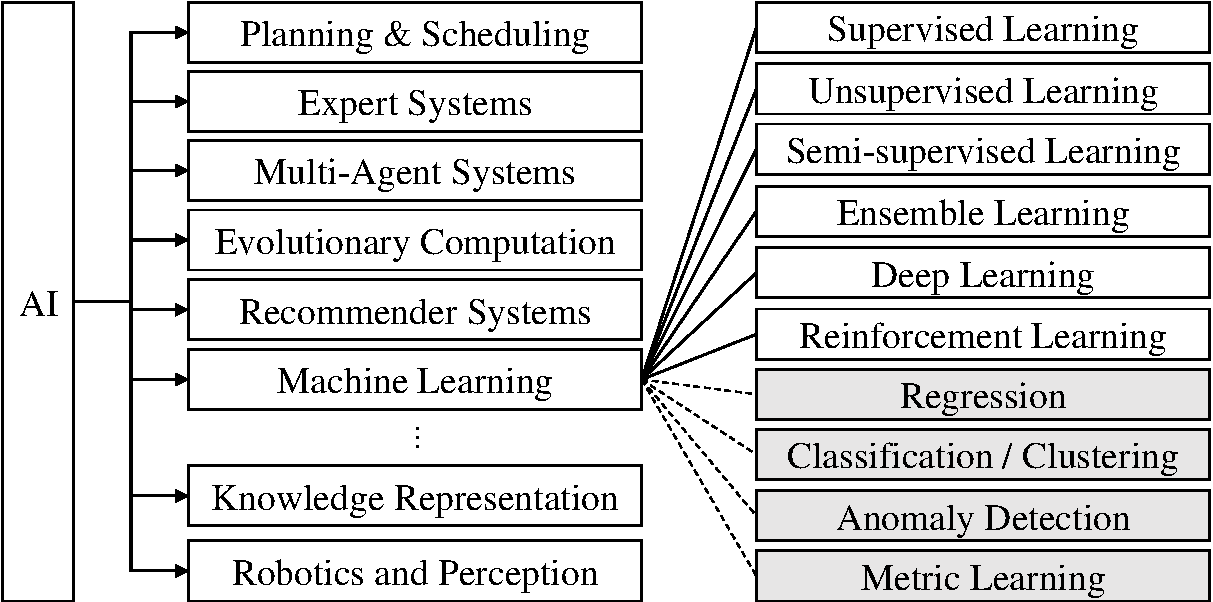
\includegraphics[width=0.7\textwidth]{Img/ai-content.pdf}
  \bicaption{人工智能研究分支}{Research branches of AI}
  \label{fig:ai}
\end{figure}

机器学习的概念起源于早期的人工智能,研究至今已有不少经典的算法:如聚类(Clustering)、决策树(Decision Tree)、Expectation Maximization (EM),朴素贝叶斯(Navie Bayes)、支持向量机(Support Vector Machine)、AdaBoost等。此外,根据算法的
学习方法不同又可分为无监督学习(如聚类等无须数据标注的)、
监督学习(如分类等需要数据标注的)、半监督学习(需要部分数据标注)、
集成学习(多个简单模型集成)、
深度学习(利用深度网络学习)和强化学习。
从上面的划分来看,深度学习属于机器学习的一个分支,而不是一个新的学习方法。只是近年来深度学习领域
的创新方法层出不穷,使得越来越多的学者都将其看作为一种独立的学习方法。
总而言之,越来越多的学者都踊跃加入深度学习研究的行列,为深度学习活跃发展及
应用做出极大的贡献。

\section{研究背景}
近些年,机器学习在人们生活的方方面面发挥着极大的作用:语音识别、交通预测、
视频监控、垃圾邮件过滤、智能客服、商品推荐等等。然而,机器学习算法需要从
大量数据集中提取有用的特征,进而做出决策,但是关于特征提取,目前并没有一个通用的方法。因此学者们提出了一个新的方法,称为表征学习
(Representation Learning),它能够在分类和检测任务中自动提取有用的
特征\cite{bengio2013representation}。
深度学习也属于一种表征学习方法,它可以提取出高维度、
高抽象的数据表征。然而,这些方法都属于监督学习,需要数据集具有清晰明确的特征,
并且每个数据样本都需要被标注。通常获取这些标注好的数据集或者去标注数据集的难度
很大。所以,越来越多的学者将重心放在无监督学习—一种无需数据标注的学习方法。在无监督学习中,
生成式模型(见\ref{sec:gm-dm}节)是相对有效的方法,早期的生成式模型
(如受限玻尔兹曼机\cite{smolensky1986information},
深度置信网络\cite{hinton2006fast}, 深度玻尔兹曼机\cite{salakhutdinov2009deep}
)
通常基于马尔可夫链、极大似然和近似推断等工具。然而这些方法的计算复杂度都很高,
并且无法保证良好的泛化性能。近年来,生成对抗网络
(Generative Adversarial Networks, GAN)\cite{goodfellow2014generative}
作为新兴的生成式模型,因其新颖的训练方式和超强的可扩展性而受到广泛关注。
%作为一种新的生成式模型受到了广泛的关注。
该模型包含生成器和判别器两个模块,
在对抗训练的过程中,生成器可以学习到数据的概率分布,同时生成一些逼真的虚假数据以迷惑判别器
,而判别器则尽可能地从虚假数据中区分出真实数据。两个网络之间通过相互对抗,
最终达到一个平衡点。值得一提的是,GAN不需要使用复杂的近似推断或马尔可夫链,
并且在计算机视觉,自然语言处理及其他众多领域都有较好的生成效果。

% 生成对抗网络最大的贡献在于它提出了一种对抗的思想。
% 这种思想已经成功应用于众多
% 领域如计算机视觉、自然语言处理等。前些年的AlphaGo\cite{silver2016mastering}打败
% 了人类顶尖围棋手的事件让AI引起了广泛关注,而AlphaGo的中间阶段就运用了对抗训练的
% 思想。对抗样本\cite{kurakin2016adversarial,athalye2018obfuscated,
% goodfellow2014explaining,kos2018adversarial}也利用了对抗的思想。
% 所谓对抗样本是指那些与真实数据
% 差别很小却被判为异常的,或者与真实数据相差很大却被判为真实类别的样本。

% GAN变体以及应用非常丰富。如前所述,GAN在不需要知道真实数据分布,
% 不需要做额外假设的情况下,可以通过随机噪声生成逼真的数据样本。这使得GAN在计算
% 机视觉和图像处理领域的应用大获成功。
GAN在图像超分辨率方面有很好的效果。SRGAN\cite{ledig2017photo}是第一个使用生成
对抗网络实现图像超分辨率的模型,ESRGAN\cite{wang2018esrgan}则通过对SRGAN的
三个主要组成部分进行改进,利用\citet{jolicoeur2018relativistic}提出
的方法令判别器输出相对的真实距离而非绝对距离。
\citet{yuan2018unsupervised}基于CycleGAN\cite{zhu2017unpaired}提出了一种无监督的图像超分辨率
方法。\citet{ding2019tgan}提出TGAN,通过探索张量结构来生成大型高质量图像。

GAN在图像生成方面也有很多应用。\citet{tran2017disentangled}提出的DR-GAN可用于姿态鲁棒的人脸识别。
\citet{huang2017beyond}提出TP-GAN模型,该模型在关注局部细节地同时还利用了整体结构,从而能够从不同角度的图片中恢复出高质量的正面视图。\citet{ma2017pose}提出了一种使用姿势指导生成人体图像的生成网络(PG$^2$),给定一个人物图像和一个姿势表征,该网络可以生成具有该姿势的该人物图像。
% \citet{cao2018learning}提出了一种基于GAN的高保真姿态不变性模型,用于生成高分辨率正面人脸。
虽然大多数研究使用GAN来合成二维图像\cite{bao2017cvae,dong2017semantic},但\citet{wu2016learning}将三维卷积应用于GAN,生成了许多三维样本包括沙发、椅子、汽车和桌子。\citet{im2016generating}使用循环对抗网络生成图像。\citet{yang2017lr}提出了分层循环生成对抗网络(LR-GAN),该模型也可以生成图像。

GAN也可以用于目标检测。考虑学习一个对变形和遮挡鲁棒的物体检测器,一个很自然的方法是使用具有变形和遮挡的数据集来训练模型。但是一些变形和遮挡非常罕见,它们甚至不会出现再现实生活中。此时可以用GAN来生成这样的数据以参与训练。\citet{wang2017fast}使用GAN生成具有变形和遮挡的实例,对手的目的是生成难以被对象检测器分类的样本。通过将segmentor和GAN相结合,Segan\cite{ehsani2018segan}能够检测到图像中被其他物体遮挡的物体。为了解决小物体检测问题,\citet{li2017perceptual}提出感知生成对抗网络模型;\citet{bai2018sod}提出了一种端到端的多任务GAN(MTGAN)。

\section{研究内容与意义}
本文研究基于生成对抗网络的分类模型。传统的分类方法如逻辑回归、支持向量机等都属于监督学习,需要数据标签,且只能应对数据量较小的情况。随着科技的飞速发展,传感器、摄像头、手机、工业设备等终端时时刻刻都在产生海量数据,对于大体量、高维度、高差异的数据,传统分类方法显得有些捉襟见肘。因此,伴随着深度学习领域的崛起,许多学者开始使用深度神经网络去做分类研究\cite{krizhevsky2012imagenet,taigman2014deepface}。在大量复杂数据面前,神经网络的超强拟合能力使其成为了挖掘数据价值的不二之选。
然而,即便使用神经网络来拟合数据,其本质也和大多数机器学习方法类似,不外乎
以下三个过程:数据压缩,特征提取和模型预测。这些过程往往依赖于大量的数据标注,但现实生活中标注好的数据十分稀缺:有些涉及隐私,有些获取代价高昂,有些甚至无法获得。因此,无监督和半监督分类成了当下的研究重点。

无监督分类通常建模为聚类问题,并且已经具有一些经典的方法:
K-means、Gaussian mixture model、Density estimation,这些方法均是针对数据分布进行建模。此外,一些判别式方法比如Maximum margin clustering (MMC)\cite{xu2005maximum}、Regularized information maximization (RIM)\cite{krause2010discriminative},则是将数据划分到某个类别,而无须估计数据分布。尽管判别式方法更为直接,但是它们容易受一些虚假相关性的影响而产生过拟合\cite{springenberg2015unsupervised}。当与深度神经网络这种拟合能力很强的模型相结合的时候,过拟合现象尤为显著。
随着深度学习的发展,基于深度模型的无监督或半监督方法也渐渐出现。它们通常训练一个生成式模型(如波尔兹曼机\cite{salakhutdinov2009deep,goodfellow2013multi}、前馈神经网络\cite{bengio2014deep,kingma2014semi}以及自编码器\cite{hinton2006reducing,vincent2008extracting}),通过重建输入样本来学习数据特征,刻画数据分布。因此,它们避免了因直接划分数据而产生的过拟合问题。但是这些方法在重建训练样本的过程中,并没有额外的约束,所以会保留原始数据的所有信息,这和训练分类器的目标相背\footnote{在训练分类器时,通常只希望保留和分类目标相关的信息,从而使得模型对其他不重要的信息更加鲁棒。}。

生成对抗网络结合了生成式和判别式模型,一定程度上克服了上述问题。通过将判别器扩展为分类器,对抗的训练机制可以让判别器无监督或半监督地学习到数据的类别特征,从而达到分类的效果。与此同时,生成器生成的数据一方面可以提高判别器的鲁棒性,一方面可以用于数据增强,进一步提升判别性能。


\section{研究现状}
在生成对抗网络的众多应用的探索过程中,不少学者研究发现GAN可以与分类模型相结合。事实上朴素GAN模型中的判别器可视为一个二分类器,给定输入样本,判别器输出该样本来自真实数据的概率,这显然可以解决二分类问题。异常检测(Anomaly Detection)某种程度上也可以看作二分类问题,所以也有不少学者将GAN用于异常检测\cite{schlegl2017unsupervised,zenati2018efficient,akcay2018ganomaly}。
对于GAN和多分类问题的结合,一个容易想到的方法是将判别器扩展为多分类器,使其输出样本属于每个类别的概率\cite{springenberg2015unsupervised,salimans2016improved}。第二种方法是利用判别器学习到的数据特征,将判别网络的中间输出作为数据特征来训练另一个分类器,通常以这种方法训练的分类器会收敛地更快并且能达到不错的分类准确率\cite{donahue2016adversarial,dumoulin2016adversarially}。

%GAN在分类问题中也有所应用\cite{springenberg2015unsupervised,salimans2016improved,odena2016semi,chongxuan2017triple,wu2019enhancing},这也是本文的研究重点。
%首先了解以下GAN做分类的基本原理。
%从未标注或仅部分标注的数据中学习非线性分类器是机器学习中长期存在的问题。它的前提是,训练数据的结构特征包含可用于推断未知标签的信息。也就是说,在无监督学习中,我们假设输入分布$p(x)$包含有关$p(y|x)$的信息,其中$y \in \Omega = \{\omega_1, \ldots, \omega_K\}$表示未知标签。通过充分利用有标签的和无标签的数据,人们希望学习出一个能够捕获到其中共性的表征。然后分类器会进一步利用这些表征,仅通过一小部分的有标签数据就能够学习到潜在数据的分布。

%- CatGAN
%- SGAN 
%- tripleGAN
%- triangleGAN
%- ETGAN
%- InfoGAN

%% from semi-supervised learning by entropy minimization
%In the probabilistic framework, semi-supervised learning can be modeled as a missing data problem, which can be addressed by generative models such as mixture models thanks to the EM algorithm and extensions thereof [6].Generative models apply to the joint density of patterns and class (X, Y ). They have appealing features, but they also have major drawbacks. Their estimation is much more demanding than discriminative models, since the model of P(X, Y ) is exhaustive, hence necessarily more complex than the model of P(Y |X). More parameters are to be estimated, resulting in more uncertainty in the estimation process. The generative model being more precise, it is also more likely to be misspecified. Finally, the fitness measure is not discriminative, so that better models are not necessarily better predictors of class labels. These difficulties have lead to proposals aiming at processing unlabeled data in the framework of supervised classification [1, 5, 11].  Here, we propose an estimation principle applicable to any probabilistic classifier, aiming at making the most of unlabeled data when they are beneficial, while providing a control on their contribution to provide robustness to the learning scheme.
%
%在概率框架中,可以将半监督学习建模为丢失的数据问题,由于EM算法及其扩展[6],可以通过生成模型(例如混合模型)来解决该问题。生成模型适用于模式的联合密度和类(X,Y)。它们具有吸引人的功能,但也有许多缺点。他们的估计比判别模型要严格得多,因为P(X,Y)模型是穷举性的,因此必定比P(Y | X)模型更复杂。要估计更多的参数,导致估计过程中更多的不确定性。生成模型更精确,也更可能被错误指定。最后,适应度度量没有区别,因此,更好的模型不一定是类别标签的更好预测指标。这些困难导致提出了旨在在监督分类框架内处理未标记数据的提议[1、5、11]。在这里,我们提出一种适用于任何概率分类器的估计原理,旨在在有益的情况下充分利用未标记的数据,同时控制其贡献,从而为学习方案提供鲁棒性

CatGAN\cite{springenberg2015unsupervised}将判别器从二分类输出扩展为多分类输出,同时设计了新的对抗目标,在MNIST\cite{lecun1989backpropagation}和CIFAR-10\cite{krizhevsky2009learning}上均取得了十分可观的分类准确率。\citet{salimans2016improved}提出了几种训练GAN的技巧,以及给出了一种半监督分类方法。不同于CatGAN,他们令判别器输出$K+1$个类别,其中$K$为数据集原始的类别个数,而多出来的类别就代表着生成器生成的虚假数据,也就是把生成器的所有输出都归为一类。这显然忽略了生成器生成的不同类别的数据。SGAN\cite{odena2016semi}提出了类似的网络模型。\citet{dai2017good}指出给定判别器的目标,良好的半监督性能需要一个较差的生成器,即对一个判别器来说,分类和区分真假是不兼容的目标。TripleGAN\cite{chongxuan2017triple}也指出了这一点,同时提出了改进方法:将分类任务和判别任务分配给两个不同的模块。具体来说,TripleGAN增加了一个分类网络,令判别器专注于区分真假,同时对训练目标做了相应改动,使得生成器和分类器对应的概率分布同时收敛到真实数据分布。\citet{wu2019enhancing}在TripleGAN的基础上应用了feature matching\cite{salimans2016improved},并且引入了两个分类网络协同工作,达到了更高的性能。
% NOTE:为什么不在improvedGAN上面扩展,加互信息呢?


\section{本文工作}
本文主要研究了两个基于生成对抗网络的分类模型,基于这两个模型提出一些算法改进。第一个模型是InfoGAN\cite{chen2016infogan},严格来说它并不属于基于GAN的分类模型,但是它包含一个辅助网络,契合了分类器的特征,因此我们可以对辅助网络添加用于分类的正则项,将辅助网络训练成一个分类器。第二个模型是CatGAN\cite{springenberg2015unsupervised},它是完全以分类为目标而设计的,因此其中有很多思想值得我们参考。例如,对于目标函数的改变,CatGAN使用判别器输出的条件分布的熵作为判别真假的依据。它创新性地引入了信息论尺度作为训练目标,在具备实践效果的同时具备一定的可解释性。

对于InfoGAN,本文几乎没有改变模型结构,通过在辅助网络的目标函数添加了一个分类损失,就达到了比较可观的分类准确率。本文称改进的模型为Classifier InfoGAN (C-InfoGAN),它保留了InfoGAN的大部分优点:比如通过离散隐变量控制生成图片的类别,以及通过连续隐变量调整生成图片的局部细节,同时还具有可观的分类性能。此外,本文还提出了半监督版本的训练方法。在拥有少量标签的情况下,可将标签直接放入辅助网络中,从而充分利用标签信息,将真实标签和隐变量相互绑定,解决了InfoGAN中离散隐变量和真实标签不对应的问题。

对于CatGAN,本文受InfoGAN启发,将生成器的输入噪声分解为无意义噪声:提供模型的容量,使得模型具有足够的自由度去学习数据的细节(高度耦合的特征);和有意义隐变量:用于在学习过程中绑定到数据类别;同时优化隐变量和生成图片之间的互信息,提出了InfoCatGAN模型。该模型可以在牺牲少量分类准确率的情况下,大大提高生成器生成图片的质量。这是由于CatGAN使用条件熵作为目标函数,没有类别指向性,因为无法从条件熵的高低推知条件分布的形态。InfoCatGAN模型通过在隐空间构造一维隐变量,在训练过程中将生成数据的类别标签与之绑定,使得可以通过该隐变量来控制生成数据的类别。改进的主要思想就是在生成虚假数据的时候,令生成器生成具体类别的数据,而不是笼统地最小化条件熵。此外,提出的模型能够很好的兼容半监督学习,并且在少量标签信息的帮助下,隐变量和真实类别一一对应,也就是说,可以通过隐变量控制生成图片的类别。

本文提出了两个改进模型都使用了基于互信息的正则项,这从侧面说明了信息论在未来的深度学习领域拥有值得探索的价值。

\section{文章结构}
本文整体章节结构安排如下:
\begin{itemize}
  \item 第一章为绪论。主要介绍本文的研究背景,即当前深度学习领域的蓬勃发展,接着介绍了本文的研究内容与意义,然后介绍了生成对抗网络的发展及众多应用,引入使用生成对抗网络模型做分类的动机和优点,介绍了国内外关于该问题的研究现状。最后概括了本文的主要工作。
  \item 第二章为预备知识。首先介绍了什么是生成式模型,什么是判别式模型,接着介绍了生成对抗网络的核心思想和基本原理。最后详细阐述了InfoGAN和CatGAN的模型结构及各自的原理和目标函数。
  \item 第三章为本文工作。分别详细介绍了本文提出的两个模型C-InfoGAN和InfoCatGAN,阐明了它们的原理以及目标函数,同时给出了训练方法。
  \item 第四章为模型评估。主要介绍了评估模型的方法和尺度,以及实验细节。接着给出了两个模型在MNIST和FashionMNIST上的结果,以及对结果做了简单分析,同时给出了模型的收敛速度。
  \item 第五章为总结与展望。对全文内容进行总结和概括,并对未来的扩展方向进行展望。
\end{itemize}
